\chapter{PENGUJIAN DAN ANALISIS}
Pada bab ini, akan dijelaskan mengenai hasil dari pengujian dan analisis dari penelitian yang telah diuraikan pada metodologi. Selain itu, akan dipaparkan mengenai skenario dari pengujian yang dilakukan untuk evaluasi performa dari sistem. Pengujian ini dilakukan untuk memastikan bahwa sistem yang telah dirancang mampu berfungsi dengan baik dan situasi yang mungkin dihadapi oleh pengguna.
\section{Skenario Pengujian}
Pengujian dilakukan untuk menguji performa dari model dalam melakukan deteksi terhadap gestur untuk sistem kendali dan sistem pengereman otomatis. Skenario pengujian dirancang untuk mengukur berbagai aspek dari sistem seperti akurasi deteksi terhadap kelas yang dipanggil, \emph{respond time}, kecepatan pemrosesan, dan respon sistem terhadap objek di depannya yang berpengaruh kepada pengereman otomatis. Skenario pengujian yang dilakukan adalah sebagai berikut;
\begin{enumerate}
    \item Hasil Pengujian model
    \item Pengujian berdasarkan FPS
    \item Pengujian berdasarkan hasil \emph{respond time}
    \item Pengujian terhadap akurasi dari kelas yang dipanggil
    \item Pengujian sistem pengereman otomatis pada jarak 150 cm
    \item Pengujian sistem pengereman otomatis pada jarak 130 cm
    \item Pengujian sistem pengereman otomatis pada jarak 100 cm
\end{enumerate}
\section{Pengujian Performa Model YOLOv11 Menggunakan Confusion Matrix}
Data yang digunakan sebagai set data berjumlah 5372 citra manusia dengan perbandingan 4359 set data train dan 1023 set data validasi. Setelah proses pemuatan set dilakukan di lanjutkan dengan proses pelatihan model.
Proses pelatihan dilakukan dengan beberapa parameter yang nantinya akan diuji, yang dimana parameter ini akan dibandingkan performanya melalui nilai confusion matrix maupun nilai akurasi deteksi seperti skor mAP, precision, box loss.
Gambar 4.1 merupakan input layer yang digunakan.
\begin{figure} [H] \centering
  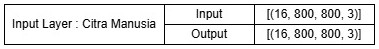
\includegraphics[scale=0.65]{gambar/Input layer.jpg}
  \caption{Input Layer Pelatihan}
  \label{fig:Pengujian Performa}
\end{figure}
Pelatihan pertama menggunakan 150 epoch. Input layer memiliki batch size sebesar 16 dengan tindakan praproses merubah ukuran gambar pada dataset menjadi 800x800 piksel. Adapun tujuan dari pelatihan ini untuk mengetahui seberapa baik peningkatan model pre- trained
yang digunakan dalam deteksi manusia berdasarkan jumlah Epoch yang ditentukan. Berikut nilai box loss yang didapatkan dari hasil training pada Gambar 4.2
\begin{figure} [H] \centering
  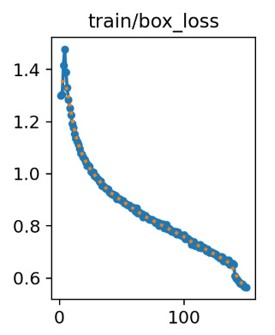
\includegraphics[scale=0.55]{gambar/train box loss.jpg}
  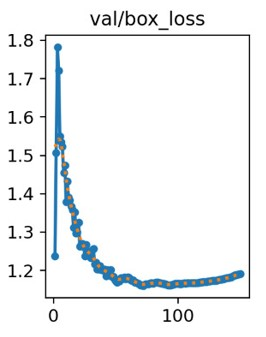
\includegraphics[scale=0.55]{gambar/val box loss.jpg}
  \caption{Grafik \emph{box loss}}
  \label{fig:Pengujian Performa}
\end{figure}
Didapatkan nilai dari \emph{box loss} pada hasil pelatihan YOLOv11 adalah sebesar 0.598
setelah 150 epoch. \emph{Box loss} mengukur seberapa baik model memprediksi bounding
box di sekitar objek. Tujuan dari loss ini adalah untuk mengoptimalkan model
agar bounding box yang diprediksi sesuai dengan posisi dan ukuran objek sebenarnya dalam gambar.
Adapun penurunan yang terlihat pada gambar pelatihan box loss menandakan bahwa hasil
pelatihan yang dilakukan telah berhasil membuat model menentukan koordinat \emph{bounding box}
pada objek manusia secara akurat.

Nilai dari \emph{box loss} pada proses validasi menggunakan YOLOv11 ini adalah 1.21,
\emph{box loss} validasi ini mengindikasi kemampuan mengenali objek pada data uji. Secara teori
, penurunan objek loss pada tahap validasi menandakan bahwa objek mampu melakukan deteksi
secara umum. Namun diakhir terlihat grafik sedikit naik. Hal ini menandakan ketika model
mulai menghafal pola data training dengan baik, tapi gagal menggeneralisasi pada data validasi.
Akibatnya, \emph{loss training} tetap atau terus menurun, loss validasi justru naik sedikit karena
model tidak mampu memprediksi data validasi dengan baik. Selanjutnya grafik dari mAP dapat dilihat
pada Gambar 4.3
\begin{figure} [H] \centering
  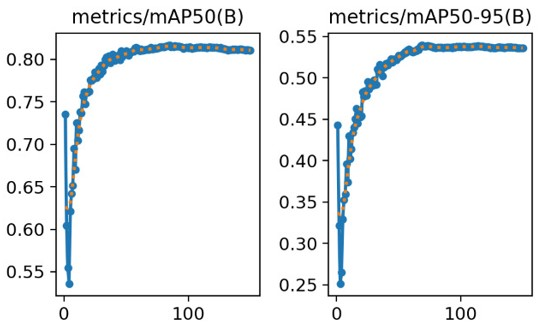
\includegraphics[scale=0.63]{gambar/map grafik yolov11.jpg}
  \caption{Grafik mAP epoch 150}
  \label{fig:Pengujian Performa}
\end{figure}
Skor mAP50 pada \emph{threshold} 0.5 yang diperoleh dari proses ini adalah sebesar 0.812, ini mengindikasikan
bahwa model memiliki kemampuan yang sangat baik dalam mendeteksi objek dengan kecepatan tinggi,
syarat minimal dari kriteria IoU adalah 0.5 terpenuhi. Hal ini menunjukan bahwa dalam percobaan kasus, \emph{bounding box}
yang diprediksi oleh model memiliki kesesuaian yang signifikan dengan \emph{bounding box ground truth}. 

Pada grafik mAP50-95 dengan prediksi yang lebih presisi. Nilai mAP50-95 adalah 0.25 diawal dan mulai terlihat kenaikan yang 
signifikan mencapai 0.543 di epoch ke 78. Hal ini menunjukan bahwa walaupun model sudah mampu mendeteksi objek dengan cukup
baik pada \emph{threshold} rendah, namun masih terdapat tantangan dalam mempertahankan akurasi deteksi
saat persyaratan presisi yang tumpang tindih semakin ketat.

Berikut merupakan grafik dari hasil yang didapatkan secara keseluruhan dari pealtihan model YOLOv11.
Pada Gambar 4.4 merupakan grafik hasil yang didapatkan pada model secara keseluruhan.
Didapatkan nilai- nilai pada masing masing grafik, pada train box loss didapatkan nilai 0.598,
pada train cls loss didapatkan nilai 0.412, pada train dfl loss didapatkan nilai 0.901 , pada
metrics precision didapatkan nilai 0.878, pada grafik recall 0.748, pada val box loss didapatkan nilai 1.211, pada val
cls loss didapatkan nilai 0.793, dan pada val dfl loss didapatkan nilai 1.342,  pada grafik mAP50
0.812, pada grafik mAP50-95 0.543

\begin{figure} [H] \centering
  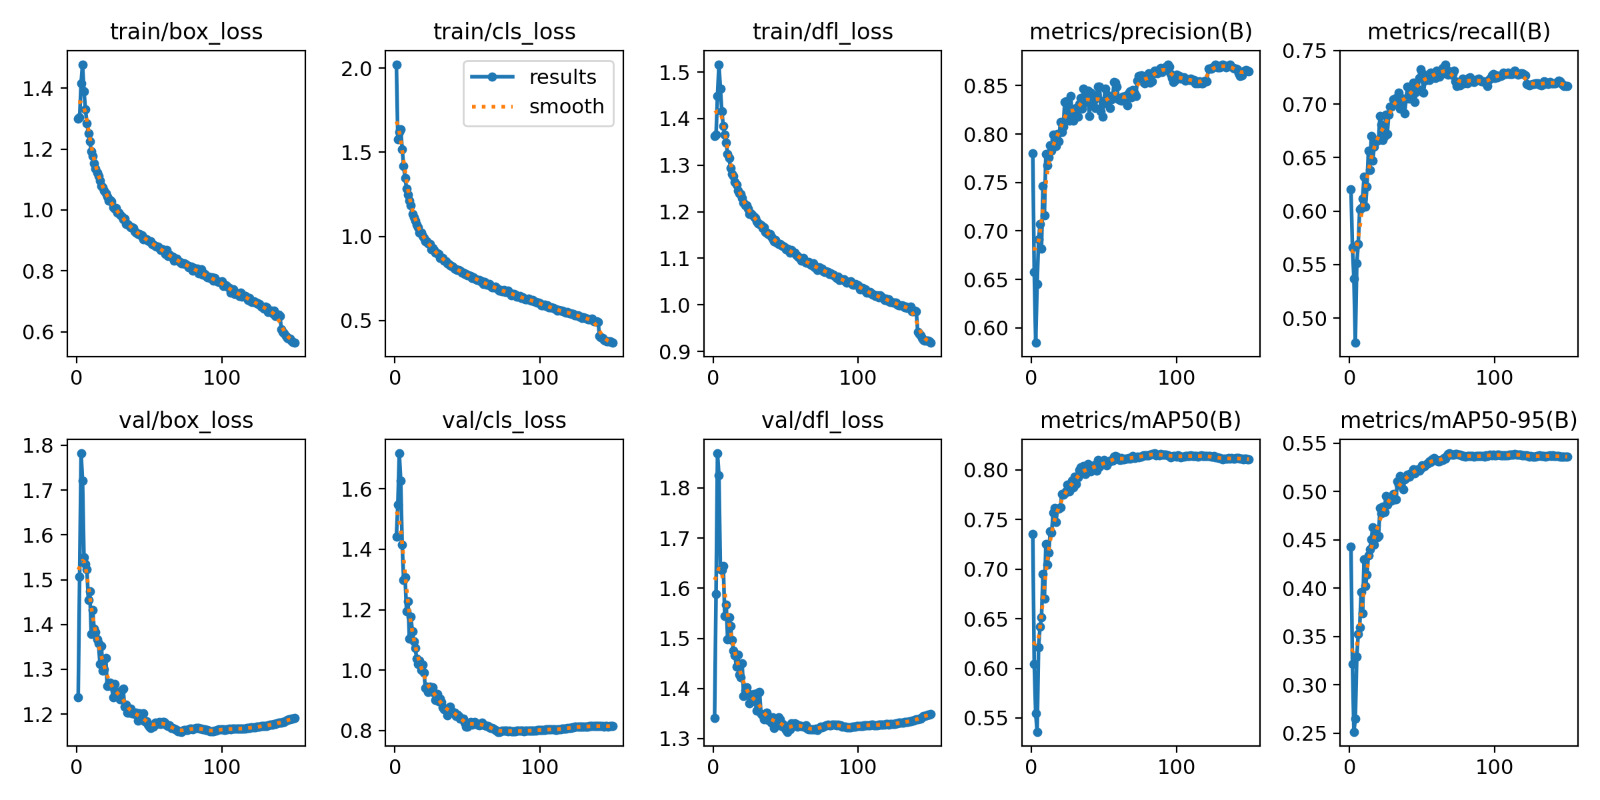
\includegraphics[scale=0.23]{gambar/Hasil.jpg}
  \caption{Grafik keseluruhan pelatihan epoch 150}
  \label{fig:Pengujian Performa}
\end{figure}

Berikut adalah visualisasi melalui \emph{confusion matrix} terkait dengan pelatihan model YOLOv11 dengan 150 epoch.
Pada Gambar 4.5 indikator yang digunakan pada \emph{confusion matrix} pada setiap kotaknya merepresentasikan nilai \emph{true positive, false positive, false negative, true negative}.
\begin{figure} [H] \centering
  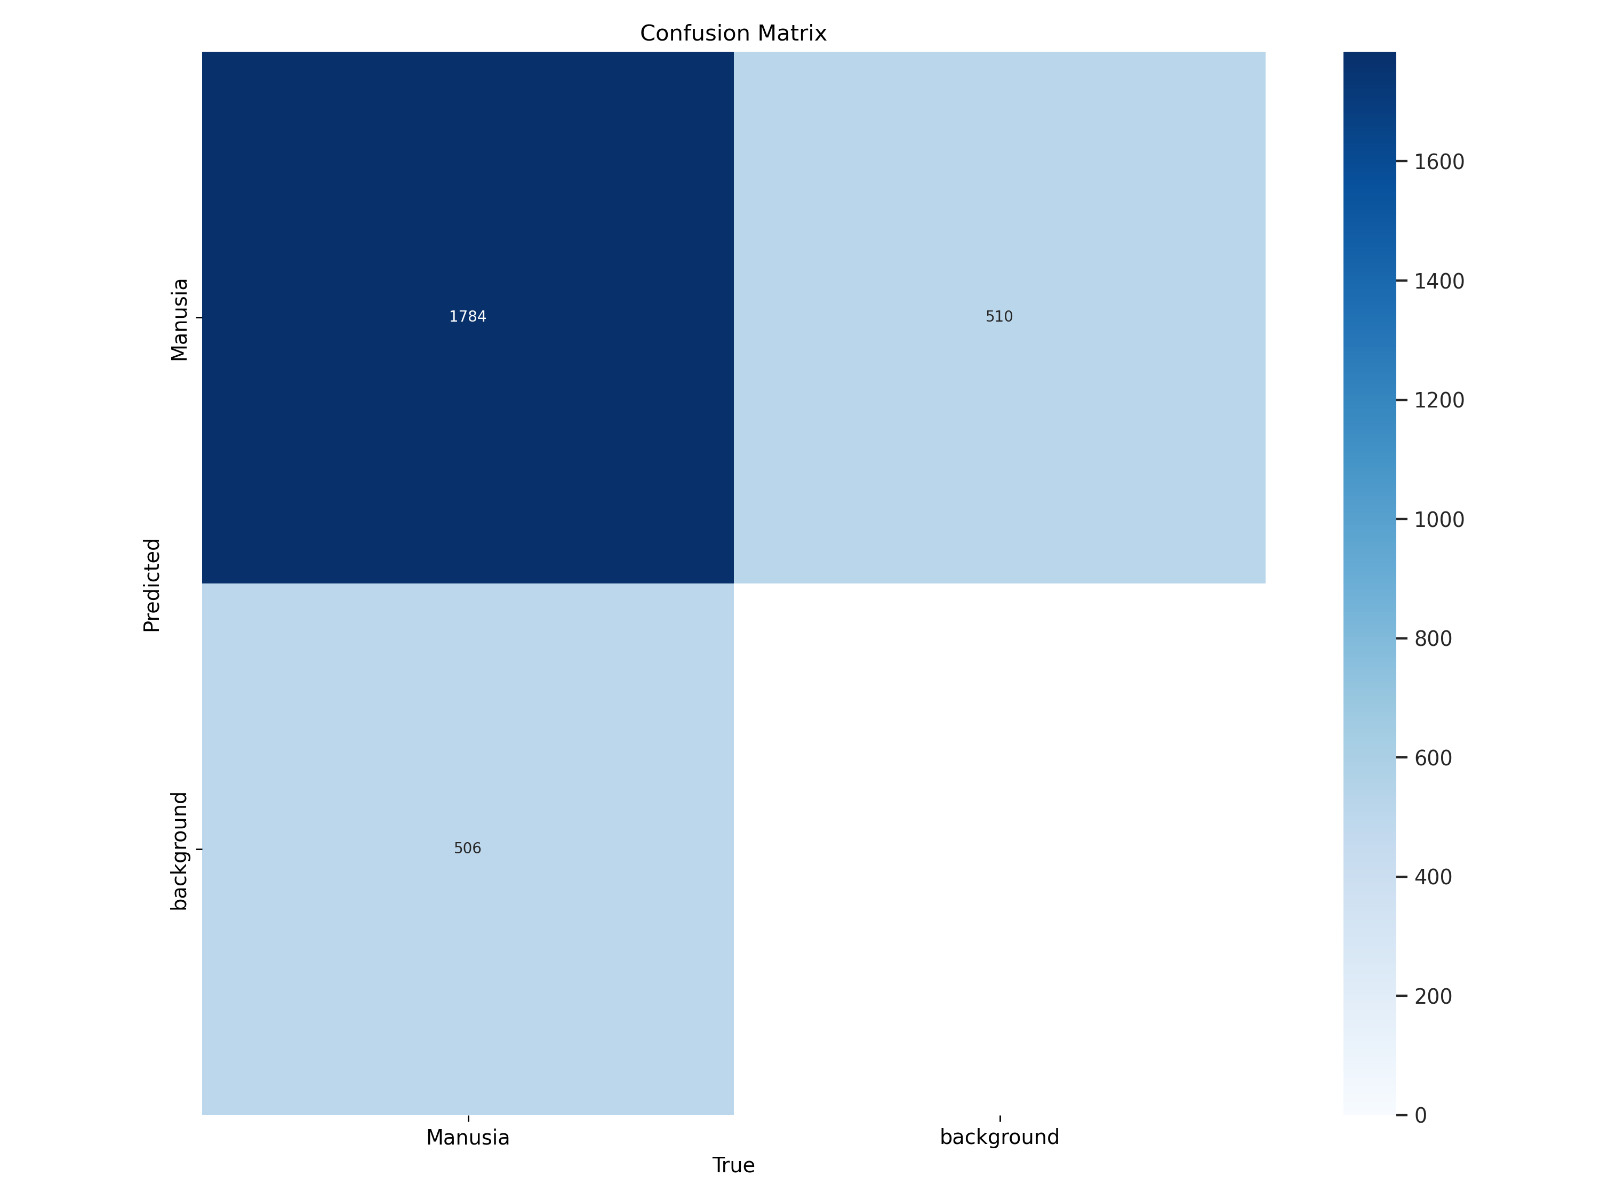
\includegraphics[scale=0.25]{gambar/Confusion matrix yolov11.jpg}
  \caption{\emph{Confusion matrix} pelatihan epoch 150}
  \label{fig:Pengujian Performa}
\end{figure}

Dari gambar 4.5 hasil pelatihan menunjukan dua kelas yakni manusia dan \emph{background}.
Dari hasil tersebut, model berhasil memprediksi hasil benar sebanyak 1784 sampel manusia. 
Namun, terdapat 510 sampel \emph{background} yang salah diklasifikasikan oleh model sebagai manusia. Disisi lain, model melewatkan 
506 sampel manusia yang diklasifikasikan sebagai \emph{background}. Selain itu, tidak ada prediksi yang benar-benar untuk kelas background,
yang mengindikasikan bahwa model cenderung memprioritaskan prediksi kelas manusia dan kurang mampu membedakan objek background dengan baik.
Hal ini menunjukkan adanya kecenderungan false positive dan false negative yang cukup signifikan

\section{Pengujian Performa Model LSTM Menggunakan Confusion Matrix}
Dataset untuk LSTM diambil dalam lima kelas dengan kelas yakni kelas kanan, stop, maju, mundur, dan kiri. Masing-masing kelas berjumlah 30 citra yang
telah di normalisasi tiap citranya, sebagai contoh pada gambar 4.6 merupakan gambar asli atau data mentah.
\begin{figure} [H] \centering
  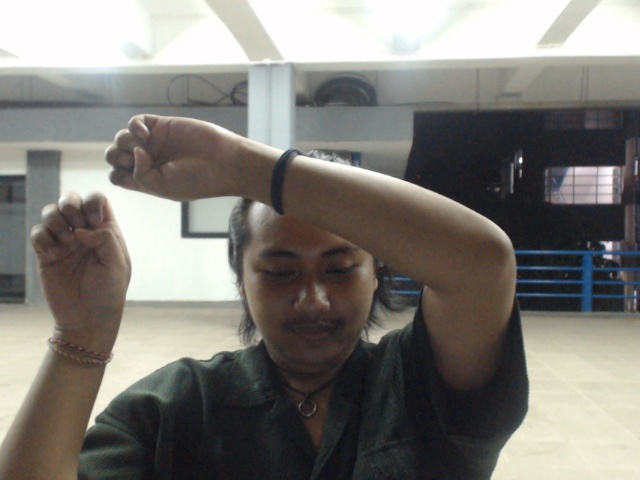
\includegraphics[scale=0.2]{gambar/0-clear.jpg}
  \caption{Dataset kelas kanan \emph{clear}}
  \label{fig:Data set kelas kanan raw}
\end{figure}

Kemudian pada gambar 4.7 menunjukan citra wajah dan tangan dengan titik-titik \emph{landmark} yang telah di deteksi menggunakan media pipe.
\begin{figure} [H] \centering
  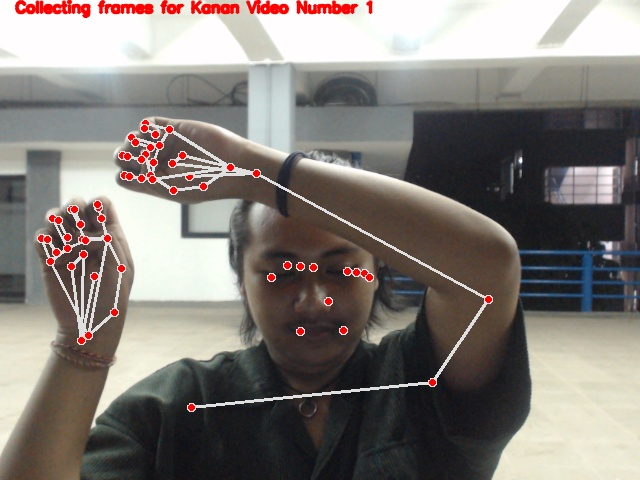
\includegraphics[scale=0.2]{gambar/1.jpg}
  \caption{Dataset kelas kanan \emph{landmark}}
  \label{fig:dataset kelas kanan clear}
\end{figure}
Dari gambar 4.7 diubah kedalam format .npy yang berisi data mentah dari titik-titik \emph{landmark}
yang terdeteksi pada bagian wajah dan dan tangan pada \emph{frame} video. File .npy ini berisi koordinat
2D dari landmark yang citra yang nantinya akan di normalisasi agar koordinat \emph{landmark} menjadi relatif 
terhadap gestur tangan sehingga data menjadi skala yang kosisten dan tidak bergantung pada ukuran asli dari citra. 
Normalisasi ini penting untuk memastikan model LSTM dapat belajar pola gestur tanpa terpengaruh perubahan ukuran citra atau posisi objek.
\begin{table}[htbp]
\centering
\caption{Tabel Sequencial}
\begin{tabular}{|l|l|l|}
\hline
\textbf{Layer (type)} & \textbf{Output Shape} & \textbf{Param \#} \\ \hline
time\_distributed (TimeDistributed) & (None, 30, 128) & 13,952 \\ \hline
lstm (LSTM) & (None, 30, 128) & 131,584 \\ \hline
dropout (Dropout) & (None, 30, 128) & 0 \\ \hline
lstm\_1 (LSTM) & (None, 30, 64) & 49,408 \\ \hline
dropout\_1 (Dropout) & (None, 30, 64) & 0 \\ \hline
lstm\_2 (LSTM) & (None, 32) & 12,416 \\ \hline
dropout\_2 (Dropout) & (None, 32) & 0 \\ \hline
dense\_1 (Dense) & (None, 16) & 528 \\ \hline
dropout\_3 (Dropout) & (None, 16) & 0 \\ \hline
dense\_2 (Dense) & (None, 16) & 272 \\ \hline
dropout\_4 (Dropout) & (None, 16) & 0 \\ \hline
dense\_3 (Dense) & (None, 5) & 85 \\ \hline
\end{tabular}
\end{table}

Tabel 4.1 menunjukkan ringkasan arsitektur model jaringan saraf yang terdiri dari beberapa layer berturut-turut. 
Dimulai dengan layer TimeDistributed yang menghasilkan output berukuran (None, 30, 128) dengan 13.952 parameter, 
yang berfungsi untuk menerapkan layer Dense pada setiap langkah waktu secara independen. Berikutnya terdapat tiga layer LSTM bertingkat, 
masing-masing dengan ukuran output (None, 30, 128), (None, 30, 64), dan (None, 32), serta jumlah parameter yang berkurang 
secara bertahap yaitu 131.584, 49.408, dan 12.416. Layer-layer ini menangani pemrosesan sekuensial data dengan mempertahankan urutan waktu 
dan mengekstrak fitur temporal yang kompleks. Setiap layer LSTM diikuti oleh layer Dropout yang tidak memiliki parameter, berfungsi sebagai 
regularisasi untuk mengurangi overfitting dengan mematikan sebagian neuron secara acak selama pelatihan. Setelah LSTM, model memiliki tiga 
layer Dense berturut-turut dengan ukuran output (None, 16), (None, 16), dan (None, 5) dengan jumlah parameter masing-masing 528, 272, dan 85. 
Layer Dense ini berfungsi untuk memetakan fitur yang telah diekstrak menjadi output klasifikasi akhir dengan 5 kelas, yang ditentukan oleh 
neuron pada layer terakhir.

Berdasarkan hasil akurasi \emph{training} yang telah dilakukan didapatkan bahwa model menghasilkan akurasi validasi bernilai 1 dan akurasi \emph{traininf}
bernilai 0.91. Data ini menunjukan peningkatan akurasi yang cukup baik pada data \emph{training} namun 
pada akurasi validasi mencapai 1.0 beberapa kali yang biasa jarang terjadi pada data validasi yang benar-benar baru dan representatif. Hal ini menandakan
data validasi terlalu kecil  atau kurang sehingga model mudah menghafal. Untuk nilai \emph{loss training} bernilai cukup tinggi di 2.56 dan \emph{loss} validasi di 
di nilai 0.05. Data ini menunjukan nilai \emph{loss training} secara umum menurun dari awal hingga akhir pelatihan, yang berarti model semakin baik dalam 
meminimalkan kesalahan terhadap data \emph{training} seiring dengan berjalannya \emph{epoch}. Untuk \emph{loss} validasi juga menunjukan tren penurunan yang konsisten. 
Hal ini mengindikasikan bahwa model dapat belajar dari data \emph{training} dengan cukup baik. Berikut merupakan grafik dari model akusari dan model \emph{loss} dari pelatihan model LSTM.
\begin{figure} [H] \centering
  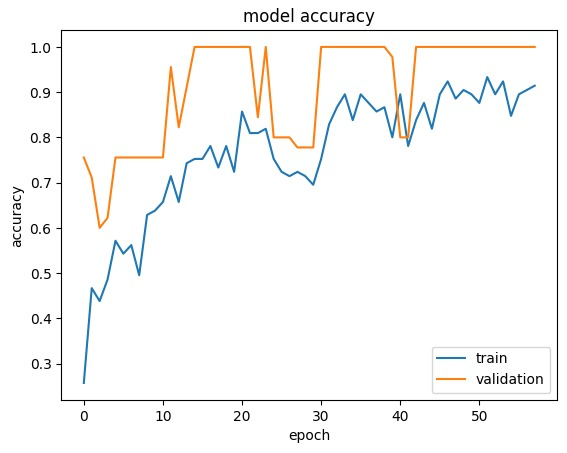
\includegraphics[scale=0.5]{gambar/akurasi model.jpg}
  \caption{Hasil \emph{accuracy} model LSTM}
  \label{fig:Pengujian Performa akurasi lstm}
\end{figure}
\begin{figure} [H] \centering
  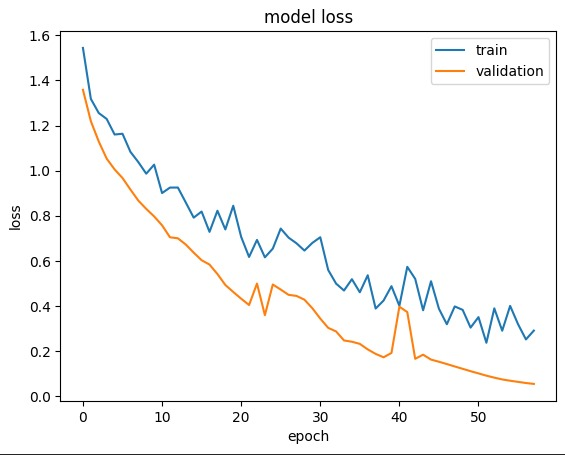
\includegraphics[scale=0.5]{gambar/akurasi loss.jpg}
  \caption{Hasil model \emph{loss} LSTM}
  \label{fig:Pengujian Performa model loss lstm}
\end{figure}

Kemudian berdasarkan model yang telah dilatih, dilakukan pengujian dengan dataset \emph{testing} yang menghasilkan \emph{confusion matrix}.
Gambar 4.10 menunjukkan confusion matrix dari sebuah model klasifikasi dengan lima kelas yaitu Stop, Maju, Mundur, Kanan, dan Kiri. Dari matriks ini dapat dilihat bahwa model mampu
mengklasifikasikan setiap kelas dengan sangat baik tanpa terjadi kesalahan prediksi antar kelas. Misalnya, untuk kelas Stop, seluruh 11 sampel diklasifikasikan dengan benar sebagai Stop, 
dan hal yang sama berlaku untuk kelas Maju dengan 11 sampel yang benar, kelas Mundur dengan 9 sampel, serta kelas Kanan dan Kiri yang masing-masing diklasifikasikan benar sebanyak 7 sampel. 
Tidak terdapat nilai selain diagonal utama yang berarti tidak ada sampel yang salah diklasifikasikan ke kelas lain. Hal ini menunjukkan performa model yang sangat akurat dalam mengenali kelima kelas tersebut. 
\begin{figure} [H] \centering
  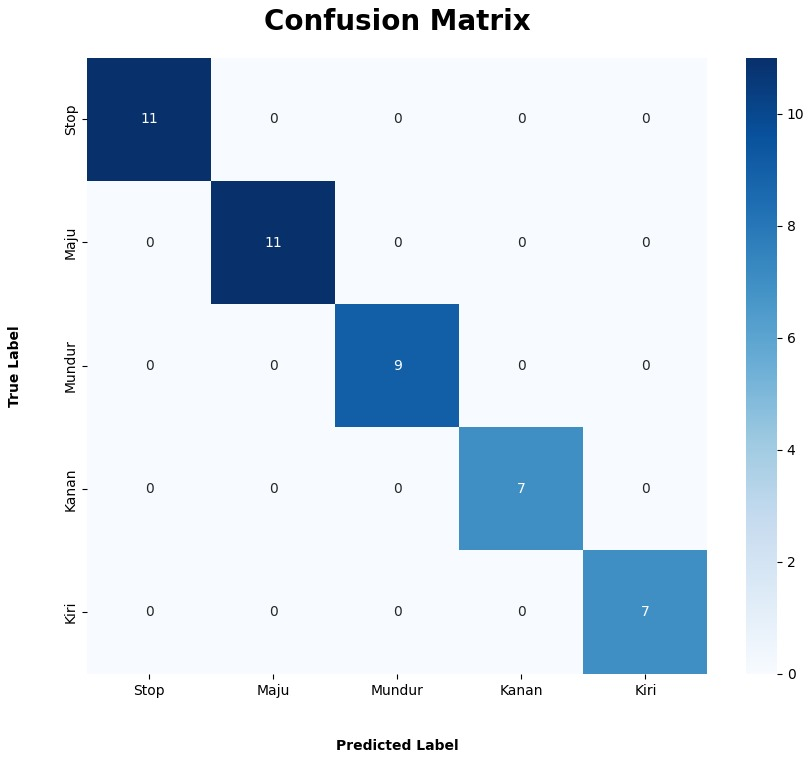
\includegraphics[scale=0.5]{gambar/confusion matrix lstm.jpg}
  \caption{Hasil \emph{confusion matrix} LSTM}
  \label{fig:Grafik confusion matrix lstm}
\end{figure}

\begin{table}[h!]
\centering
\caption{Classification Report}
\begin{tabular}{lcccc}
\hline
\textbf{Class} & \textbf{Precision} & \textbf{Recall} & \textbf{F1-score} & \textbf{Support} \\
\hline
Stop   & 1.00 & 1.00 & 1.00 & 11 \\
Maju   & 1.00 & 1.00 & 1.00 & 11 \\
Mundur & 1.00 & 1.00 & 1.00 & 9  \\
Kanan  & 1.00 & 1.00 & 1.00 & 7  \\
Kiri   & 1.00 & 1.00 & 1.00 & 7  \\
\hline
\textbf{Accuracy}     & \multicolumn{4}{c}{1.00} \\
\textbf{Macro avg}    & 1.00 & 1.00 & 1.00 & 45 \\
\textbf{Weighted avg} & 1.00 & 1.00 & 1.00 & 45 \\
\hline
\end{tabular}
\end{table}

Tabel 4.2 menunjukkan hasil evaluasi model klasifikasi untuk lima kelas, yaitu Stop, Maju, Mundur, Kanan, dan Kiri. Dari tabel tersebut terlihat bahwa model mencapai nilai precision, recall, dan f1-score sebesar 1.00 pada semua kelas, 
yang berarti model mampu mengklasifikasikan setiap kelas dengan sempurna tanpa kesalahan. Support menunjukkan jumlah data uji pada masing-masing kelas, dengan total 45 sampel yang tersebar di kelima kelas tersebut. Nilai accuracy sebesar 1.00 
mengindikasikan bahwa model memiliki akurasi 100\% secara keseluruhan pada data uji ini. Selain itu, nilai macro average dan weighted average yang juga 1.00 memperkuat bahwa performa model sangat baik dan konsisten di seluruh kelas.

\section{Pengujian Berdasarkan FPS}
Pengujian FPS akan dilakukan pada dua device yang pertama adalah pengujian pada device Laptop, dan pengujian pada device NUC. Dalam pengujian ini akan diambil nilai FPS sebanyak 30 kali yang sesuai dengan output sistem dan sudah diolah pada bagian sebelumnya.

Pada pengujian ini akan diambil nilai FPS pada laptop dan FPS pada NUC. Spesifikasi laptop yang digunakan untuk pengujian ini pada tabel  :

\begin{longtable}{|c|c|}
  \caption{Spesifikasi Laptop}
  \label{tb:Spesifikasi Laptop}                                   \\
  \hline
  \rowcolor[HTML]{C0C0C0}
  \textbf{Komponen} & \textbf{Spesifikasi}  \\
  \hline
  CPU            & Intel(R) Core(TM) i5-10300H CPU @2.50GHz(8CPU)        \\ \hline
  RAM            & 16 GB DDR4-2666 SDRAM        \\ \hline
  GPU            & NVIDIA® GeForce RTX™ 2060 with Max-Q design           \\ \hline
  \hline
\end{longtable}

Spesifikasi NUC yang digunakan untuk pengujian ini pada tabel  :

\begin{longtable}{|c|c|}
    \caption{Spesifikasi NUC}
    \label{tb:Spesifikasi NUC}                             \\
    \hline   
    \rowcolor[HTML]{C0C0C0}
    \textbf{Komponen} & \textbf{Spesifikasi} \\
    \hline
  CPU            &  Intel® Core™ i7-1165G7        \\
  RAM            & 32 GBLPDDR4        \\
  OS            & Windows 11 Home Single Language           \\
  \hline
\end{longtable}

Baik system kontrol maupun system pengereman otomatis akan diambil nilai fpsnya, selain itu setiap jenis arsitektur YOLO juga akan dibandingkan untuk menilai efisiensi sistem berdasarkan jenis arsitektur YOLO yang digunakan. Pengujian ini dilakukan dengan cara menjalankan sistem pada laptop dan NUC, kemudian merekam hasil dari pengujian tersebut. Hasil dari pengujian ini akan ditampilkan dalam bentuk tabel.

\newpage

\subsection{Pengujian Model YOLOv11 Berdasarkan FPS pada Laptop}

Pengujian dilakukan pada laptop dengan spesifikasi yang telah disebutkan sebelumnya. Pengujian ini dilakukan dengan cara menjalankan sistem pada laptop dan merekam hasil dari pengujian tersebut. Hasil dari pengujian ini akan ditampilkan dalam bentuk tabel. Gambar \ref{fig:Foto pengujian fps laptop} merupakan gambar pengambilan data fps pada laptop.

\begin{figure} [H] \centering
  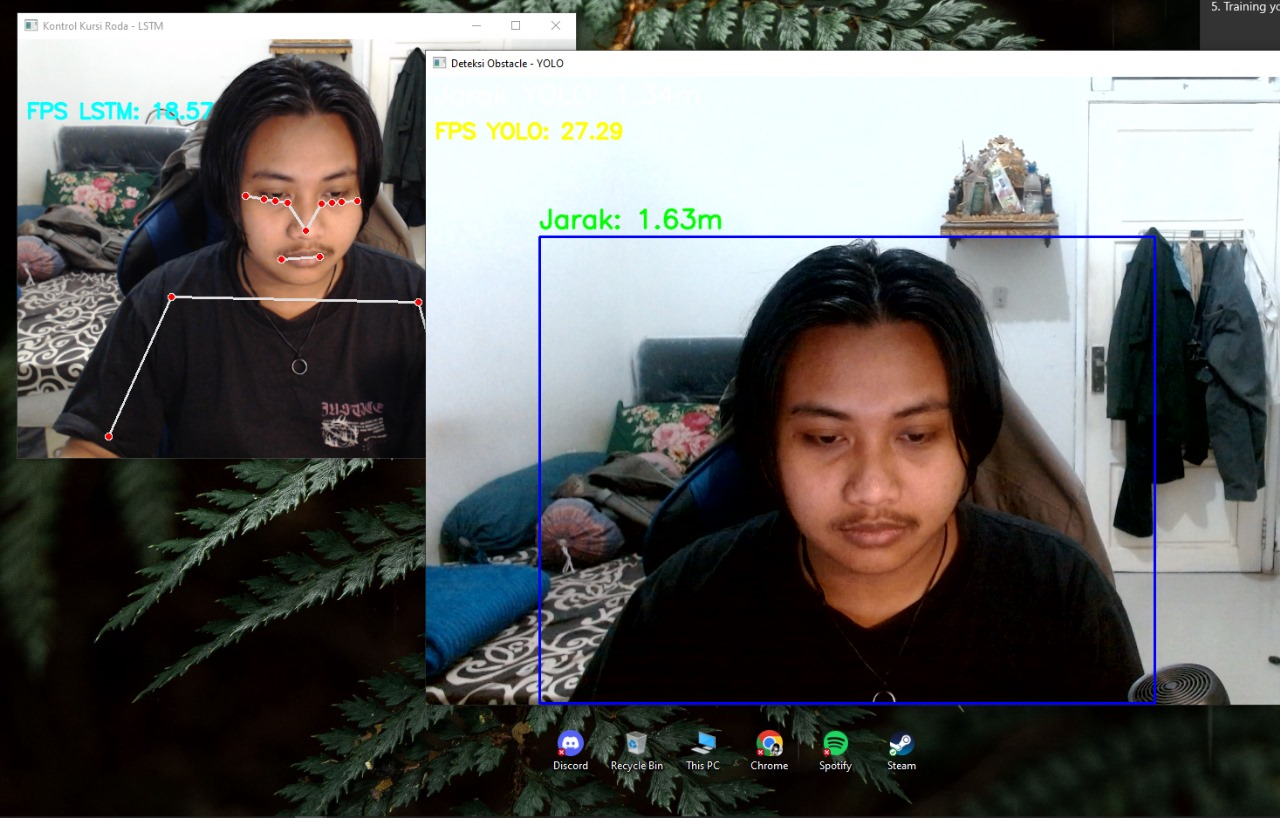
\includegraphics[scale=0.3]{gambar/devafps.jpg}
  \caption{Pengujian FPS pada Laptop}
  \label{fig:Foto pengujian fps laptop}
\end{figure}

Pada tabel \ref{tb:TabelYolov11Laptop} merupakan hasil dari pengujian model YOLOv11 berdasarkan FPS pada Laptop. Dari hasil tersebut didapatkan rata rata FPS sebesar 24,969 , dengan nilai tertinggi FPS sebesar 35,81 dan nilai terendah sebesar 12,8.

\begin{table}[H]
  \caption{Nilai Pengujian Model YOLOv11 Berdasarkan FPS pada Laptop} 
  \label{tb:TabelYolov11Laptop}
  \centering
  \begin{tabular}{|l|l|l|l|l|l|l|l|}
  \cline{1-2} \cline{4-5} \cline{7-8}
  No & FPS   &  & No & FPS   &  & No & FPS   \\ \cline{1-2} \cline{4-5} \cline{7-8} 
  1  & 21,8  &  & 11 & 21,82 &  & 21 & 23,32 \\ \cline{1-2} \cline{4-5} \cline{7-8} 
  2  & 20,89 &  & 12 & 20,89 &  & 22 & 23,89 \\ \cline{1-2} \cline{4-5} \cline{7-8} 
  3  & 25,7  &  & 13 & 17,9  &  & 23 & 21,18 \\ \cline{1-2} \cline{4-5} \cline{7-8} 
  4  & 12,8  &  & 14 & 23,57 &  & 24 & 31,33 \\ \cline{1-2} \cline{4-5} \cline{7-8} 
  5  & 23,32 &  & 15 & 21,77 &  & 25 & 30,38 \\ \cline{1-2} \cline{4-5} \cline{7-8} 
  6  & 34,57 &  & 16 & 17,34 &  & 26 & 29,49 \\ \cline{1-2} \cline{4-5} \cline{7-8} 
  7  & 21,33 &  & 17 & 26,39 &  & 27 & 33,42 \\ \cline{1-2} \cline{4-5} \cline{7-8} 
  8  & 35,81 &  & 18 & 19,28 &  & 28 & 32,34 \\ \cline{1-2} \cline{4-5} \cline{7-8} 
  9  & 21,8  &  & 19 & 32,34 &  & 29 & 28,31 \\ \cline{1-2} \cline{4-5} \cline{7-8} 
  10 & 24,45 &  & 20 & 29,54 &  & 30 & 22,12 \\ \cline{1-2} \cline{4-5} \cline{7-8} 
  \end{tabular}
  \end{table}

Pada pengujian menggunakan model YOLOv11 pada laptop ini, hasil yang didapatkan sangat baik dimana FPS menyentuh angka yang cukup tinggi. Hal ini menunjukan bahwa sistem dapat berjalan dengan baik dan efisien. Adapun ketidak stabilan pada FPS disebabkan oleh beberapa faktor seperti banyaknya objek yang terdeteksi, dan juga pengaruh dari suhu laptop selama pengujian. 

\subsection{Pengujian Model YOLOv8 Berdasarkan FPS pada Laptop}

Pengujian dilakukan pada laptop dengan spesifikasi yang telah disebutkan sebelumnya. Pengujian ini dilakukan dengan cara menjalankan sistem pada laptop dan merekam hasil dari pengujian tersebut. Hasil dari pengujian ini akan ditampilkan dalam bentuk tabel. 

Pada tabel \ref{tb:TabelYolov8Laptop} merupakan hasil dari pengujian model YOLOv8 berdasarkan FPS pada Laptop. Dari hasil tersebut didapatkan rata rata FPS sebesar 6,782, dengan nilai tertinggi FPS sebesar 8,89 dan nilai terendah sebesar 4,12.

\begin{table}[H]
  \caption{Nilai Pengujian Model YOLOv8 Berdasarkan FPS pada Laptop} 
  \label{tb:TabelYolov8Laptop}
  \centering
  \begin{tabular}{|l|l|l|l|l|l|l|l|}
  \cline{1-2} \cline{4-5} \cline{7-8}
  No & FPS  &  & No & FPS  &  & No & FPS  \\ \cline{1-2} \cline{4-5} \cline{7-8} 
  1  & 6,68 &  & 11 & 6,24 &  & 21 & 5,12 \\ \cline{1-2} \cline{4-5} \cline{7-8} 
  2  & 7,43 &  & 12 & 4,77 &  & 22 & 8,43 \\ \cline{1-2} \cline{4-5} \cline{7-8} 
  3  & 6,68 &  & 13 & 7,43 &  & 23 & 6,73 \\ \cline{1-2} \cline{4-5} \cline{7-8} 
  4  & 8,89 &  & 14 & 8,36 &  & 24 & 8,36 \\ \cline{1-2} \cline{4-5} \cline{7-8} 
  5  & 6,08 &  & 15 & 6,68 &  & 25 & 6,43 \\ \cline{1-2} \cline{4-5} \cline{7-8} 
  6  & 7,43 &  & 16 & 7,23 &  & 26 & 5,33 \\ \cline{1-2} \cline{4-5} \cline{7-8} 
  7  & 8,36 &  & 17 & 4,12 &  & 27 & 6,59 \\ \cline{1-2} \cline{4-5} \cline{7-8} 
  8  & 5,12 &  & 18 & 6,88 &  & 28 & 7,1  \\ \cline{1-2} \cline{4-5} \cline{7-8} 
  9  & 6,14 &  & 19 & 7,48 &  & 29 & 5,43 \\ \cline{1-2} \cline{4-5} \cline{7-8} 
  10 & 7,87 &  & 20 & 7,42 &  & 30 & 6,65 \\ \cline{1-2} \cline{4-5} \cline{7-8} 
  \end{tabular}
  \end{table}

Pada pengujian menggunakan model YOLOv8 pada laptop ini, hasil yang didapatkan kurang baik dimana FPS menyentuh angka yang cukup rendah. Hal ini menunjukan bahwa sistem dapat berjalan dengan baik namun tidak efisien.

\subsection{Pengujian Model YOLOv12 Berdasarkan FPS pada Laptop}

Pengujian dilakukan pada laptop dengan spesifikasi yang telah disebutkan sebelumnya. Pengujian ini dilakukan dengan cara menjalankan sistem pada laptop dan merekam hasil dari pengujian tersebut. Hasil dari pengujian ini akan ditampilkan dalam bentuk tabel. Gambar \ref{fig:Foto pengujian fps laptop} merupakan gambar pengambilan data fps pada laptop.

Pada tabel \ref{tb:TabelYolov12xLaptop} merupakan hasil dari pengujian model YOLOv8 berdasarkan FPS pada Laptop. Dari hasil tersebut didapatkan rata rata FPS sebesar 27.xxx, dengan nilai tertinggi FPS sebesar 30.xxx dan nilai terendah sebesar 19.xxx.

\begin{table}[H]
  \centering
  \caption{Nilai Pengujian Model YOLOv12 Berdasarkan FPS pada Laptop} 
  \label{tb:TabelYolov12xLaptop}
  \begin{tabular}{|l|l|l|l|l|l|l|l|}
  \cline{1-2} \cline{4-5} \cline{7-8}
  No & FPS &  & No & FPS &  & No & FPS \\ \cline{1-2} \cline{4-5} \cline{7-8} 
  1  &     &  & 11 &     &  & 21 &     \\ \cline{1-2} \cline{4-5} \cline{7-8} 
  2  &     &  & 12 &     &  & 22 &     \\ \cline{1-2} \cline{4-5} \cline{7-8} 
  3  &     &  & 13 &     &  & 23 &     \\ \cline{1-2} \cline{4-5} \cline{7-8} 
  4  &     &  & 14 &     &  & 24 &     \\ \cline{1-2} \cline{4-5} \cline{7-8} 
  5  &     &  & 15 &     &  & 25 &     \\ \cline{1-2} \cline{4-5} \cline{7-8} 
  6  &     &  & 16 &     &  & 26 &     \\ \cline{1-2} \cline{4-5} \cline{7-8} 
  7  &     &  & 17 &     &  & 27 &     \\ \cline{1-2} \cline{4-5} \cline{7-8} 
  8  &     &  & 18 &     &  & 28 &     \\ \cline{1-2} \cline{4-5} \cline{7-8} 
  9  &     &  & 19 &     &  & 29 &     \\ \cline{1-2} \cline{4-5} \cline{7-8} 
  10 &     &  & 20 &     &  & 30 &     \\ \cline{1-2} \cline{4-5} \cline{7-8} 
  \end{tabular}
  \end{table}

Pada pengujian menggunakan model YOLOv12 pada laptop ini, hasil yang didapatkan sangat baik dimana FPS menyentuh angka yang cukup tinggi. Hal ini menunjukan bahwa sistem dapat berjalan dengan baik dan efisien, hal ini akan menjadi sangat penting bahwa output dari model YOLOv12 akan menjadi variabel utama dalam sistem pengereman otomatis.

\subsection{Pengujian Model LSTM Berdasarkan FPS pada Laptop}

Pengujian dilakukan pada laptop dengan spesifikasi yang telah disebutkan sebelumnya. Pengujian ini dilakukan dengan cara menjalankan sistem pada laptop dan merekam hasil dari pengujian tersebut. Hasil dari pengujian ini akan ditampilkan dalam bentuk tabel.

Pada tabel \ref{tb:TabelLSTMLaptop} merupakan hasil dari pengujian model LSTM berdasarkan FPS pada Laptop. Dari hasil tersebut didapatkan rata rata FPS sebesar 23,813 , dengan nilai tertinggi FPS sebesar 26,32 dan nilai terendah sebesar 22,19.


\begin{table}[H]
  \centering
  \caption{Nilai Pengujian Model LSTM Berdasarkan FPS pada Laptop} 
  \label{tb:TabelLSTMLaptop}
  \begin{tabular}{|l|l|l|l|l|l|l|l|}
  \cline{1-2} \cline{4-5} \cline{7-8}
  No & FPS   &  & No & FPS   &  & No & FPS   \\ \cline{1-2} \cline{4-5} \cline{7-8} 
  1  & 25,91 &  & 11 & 23,09 &  & 21 & 22,38 \\ \cline{1-2} \cline{4-5} \cline{7-8} 
  2  & 22,43 &  & 12 & 24,67 &  & 22 & 22,79 \\ \cline{1-2} \cline{4-5} \cline{7-8} 
  3  & 23,25 &  & 13 & 22,76 &  & 23 & 24,57 \\ \cline{1-2} \cline{4-5} \cline{7-8} 
  4  & 23,98 &  & 14 & 25,74 &  & 24 & 22,73 \\ \cline{1-2} \cline{4-5} \cline{7-8} 
  5  & 26,32 &  & 15 & 23,46 &  & 25 & 22,62 \\ \cline{1-2} \cline{4-5} \cline{7-8} 
  6  & 22,19 &  & 16 & 25,3  &  & 26 & 25,03 \\ \cline{1-2} \cline{4-5} \cline{7-8} 
  7  & 23,32 &  & 17 & 25,96 &  & 27 & 23,17 \\ \cline{1-2} \cline{4-5} \cline{7-8} 
  8  & 22,57 &  & 18 & 22,51 &  & 28 & 25,16 \\ \cline{1-2} \cline{4-5} \cline{7-8} 
  9  & 22,76 &  & 19 & 24,97 &  & 29 & 25,06 \\ \cline{1-2} \cline{4-5} \cline{7-8} 
  10 & 24,78 &  & 20 & 22,43 &  & 30 & 22,48 \\ \cline{1-2} \cline{4-5} \cline{7-8} 
  \end{tabular}
\end{table}

Pada pengujian menggunakan model LSTM pada laptop ini, hasil yang didapatkan sangat baik dimana FPS menyentuh angka yang cukup tinggi. Hal ini menunjukan bahwa sistem dapat berjalan dengan baik dan efisien, hal ini akan menjadi sangat penting bahwa output klasifikasi gestur dari model LSTM akan digunakan dalam sistem kendali kursi roda. FPS yang didapatkan cendrung stabil tanpa drop yang signifikan, hal ini menunjukan bahwa sistem dapat berjalan dengan baik dan efisien.


\subsection{Pengujian Model YOLOv11 Berdasarkan FPS pada NUC}

Pengujian dilakukan pada NUC dengan spesifikasi yang telah disebutkan sebelumnya. Pengujian ini dilakukan dengan cara menjalankan sistem pada NUC dan merekam hasil dari pengujian tersebut. Hasil dari pengujian ini akan ditampilkan dalam bentuk tabel. Gambar \ref{fig:Foto pengujian fps NUC} merupakan gambar pengambilan data fps pada NUC.

\begin{figure} [H] \centering
  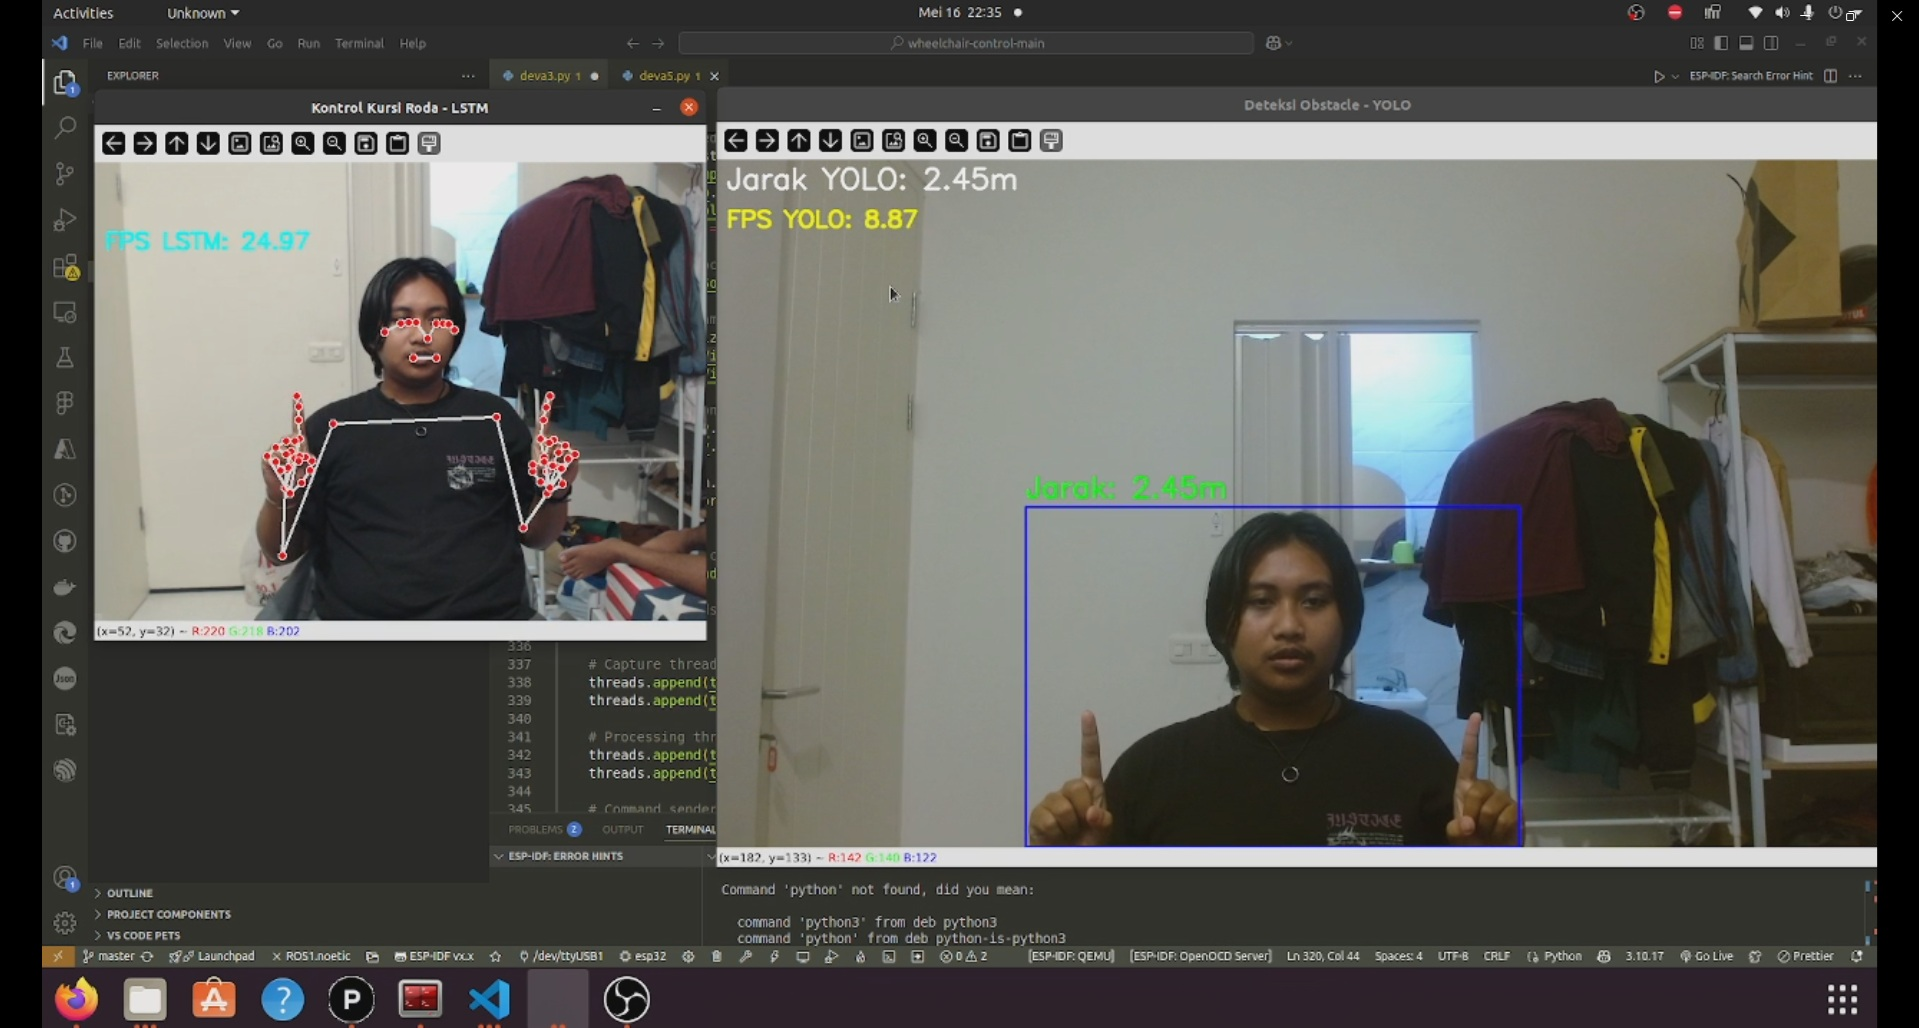
\includegraphics[scale=0.3]{gambar/v8devanuc.jpg}
  \caption{Pengujian FPS pada NUC}
  \label{fig:Foto pengujian fps NUC}
\end{figure}

Pada tabel \ref{tb:TabelYolov11NUC} merupakan hasil dari pengujian model YOLOv11 berdasarkan FPS pada NUC. Dari hasil tersebut didapatkan rata rata FPS sebesar 10,042, dengan nilai tertinggi FPS sebesar 11,21 dan nilai terendah sebesar 9,12.

\begin{table}[H]
  \caption{Nilai Pengujian Model YOLOv11 Berdasarkan FPS pada NUC} 
  \label{tb:TabelYolov11NUC}
  \centering
  \begin{tabular}{|l|l|l|l|l|l|l|l|}
  \cline{1-2} \cline{4-5} \cline{7-8}
  No & FPS   &  & No & FPS   &  & No & FPS   \\ \cline{1-2} \cline{4-5} \cline{7-8} 
  1  & 9,12  &  & 11 & 10,4  &  & 21 & 9,59  \\ \cline{1-2} \cline{4-5} \cline{7-8} 
  2  & 10,02 &  & 12 & 11,21 &  & 22 & 9,97  \\ \cline{1-2} \cline{4-5} \cline{7-8} 
  3  & 10    &  & 13 & 10,87 &  & 23 & 10,09 \\ \cline{1-2} \cline{4-5} \cline{7-8} 
  4  & 9,94  &  & 14 & 9,87  &  & 24 & 9,97  \\ \cline{1-2} \cline{4-5} \cline{7-8} 
  5  & 10,28 &  & 15 & 9,23  &  & 25 & 10,21 \\ \cline{1-2} \cline{4-5} \cline{7-8} 
  6  & 9,54  &  & 16 & 10,65 &  & 26 & 9,89  \\ \cline{1-2} \cline{4-5} \cline{7-8} 
  7  & 9,95  &  & 17 & 10,02 &  & 27 & 10    \\ \cline{1-2} \cline{4-5} \cline{7-8} 
  8  & 9,86  &  & 18 & 9,92  &  & 28 & 10,19 \\ \cline{1-2} \cline{4-5} \cline{7-8} 
  9  & 10,32 &  & 19 & 10,03 &  & 29 & 10,22 \\ \cline{1-2} \cline{4-5} \cline{7-8} 
  10 & 9,94  &  & 20 & 10,09 &  & 30 & 9,87  \\ \cline{1-2} \cline{4-5} \cline{7-8} 
  \end{tabular}
\end{table}

Pada pengujian menggunakan model YOLOv11 pada NUC ini, hasil yang didapatkan sangat baik dimana FPS menyentuh angka yang cukup tinggi. Hal ini menunjukan bahwa sistem dapat berjalan dengan baik dan efisien.

\subsection{Pengujian Model YOLOv8 Berdasarkan FPS pada NUC}

Pengujian dilakukan pada NUC dengan spesifikasi yang telah disebutkan sebelumnya. Pengujian ini dilakukan dengan cara menjalankan sistem pada NUC dan merekam hasil dari pengujian tersebut. Hasil dari pengujian ini akan ditampilkan dalam bentuk tabel.

Pada tabel \ref{tb:TabelYolov8NUC} merupakan hasil dari pengujian model YOLOv8 berdasarkan FPS pada NUC. Dari hasil tersebut didapatkan rata rata FPS sebesar 5,616 , dengan nilai tertinggi FPS sebesar 7,33 dan nilai terendah sebesar 3,65.

\begin{table}[H]
  \caption{Nilai Pengujian Model YOLOv8 Berdasarkan FPS pada NUC} 
  \label{tb:TabelYolov8NUC}
  \centering
  \begin{tabular}{|l|l|l|l|l|l|l|l|}
  \cline{1-2} \cline{4-5} \cline{7-8}
  No & FPS  &  & No & FPS  &  & No & FPS  \\ \cline{1-2} \cline{4-5} \cline{7-8} 
  1  & 5,43 &  & 11 & 6,34 &  & 21 & 5,32 \\ \cline{1-2} \cline{4-5} \cline{7-8} 
  2  & 3,65 &  & 12 & 5,76 &  & 22 & 6,43 \\ \cline{1-2} \cline{4-5} \cline{7-8} 
  3  & 5,67 &  & 13 & 5,98 &  & 23 & 5,65 \\ \cline{1-2} \cline{4-5} \cline{7-8} 
  4  & 6,54 &  & 14 & 5,34 &  & 24 & 6,19 \\ \cline{1-2} \cline{4-5} \cline{7-8} 
  5  & 5,34 &  & 15 & 6,32 &  & 25 & 5,71 \\ \cline{1-2} \cline{4-5} \cline{7-8} 
  6  & 4,98 &  & 16 & 4,94 &  & 26 & 4,31 \\ \cline{1-2} \cline{4-5} \cline{7-8} 
  7  & 5,74 &  & 17 & 5,53 &  & 27 & 4,67 \\ \cline{1-2} \cline{4-5} \cline{7-8} 
  8  & 5,01 &  & 18 & 5,67 &  & 28 & 5,43 \\ \cline{1-2} \cline{4-5} \cline{7-8} 
  9  & 6,43 &  & 19 & 6,32 &  & 29 & 4,81 \\ \cline{1-2} \cline{4-5} \cline{7-8} 
  10 & 7,33 &  & 20 & 5,12 &  & 30 & 6,53 \\ \cline{1-2} \cline{4-5} \cline{7-8} 
  \end{tabular}
\end{table}

Pada pengujian menggunakan model YOLOv8 pada NUC ini, hasil yang didapatkan kurang baik dimana FPS menyentuh angka yang cukup rendah. Hal ini menunjukan bahwa sistem dapat berjalan dengan baik namun tidak efisien.

\subsection{Pengujian Model YOLOv12 Berdasarkan FPS pada NUC}

Pengujian dilakukan pada NUC dengan spesifikasi yang telah disebutkan sebelumnya. Pengujian ini dilakukan dengan cara menjalankan sistem pada NUC dan merekam hasil dari pengujian tersebut. Hasil dari pengujian ini akan ditampilkan dalam bentuk tabel. 

Pada tabel \ref{tb:TabelYoloLaptop} merupakan hasil dari pengujian model YOLOv12 berdasarkan FPS pada NUC. Dari hasil tersebut didapatkan rata rata FPS sebesar 27.xxx, dengan nilai tertinggi FPS sebesar 30.xxx dan nilai terendah sebesar 19.xxx.

\begin{table}[H]
  \centering
  \caption{Nilai Pengujian Model YOLOv12 Berdasarkan FPS pada NUC} 
  \label{tb:TabelYolov12Nuc}
  \begin{tabular}{|l|l|l|l|l|l|l|l|}
  \cline{1-2} \cline{4-5} \cline{7-8}
  No & FPS &  & No & FPS &  & No & FPS \\ \cline{1-2} \cline{4-5} \cline{7-8} 
  1  &     &  & 11 &     &  & 21 &     \\ \cline{1-2} \cline{4-5} \cline{7-8} 
  2  &     &  & 12 &     &  & 22 &     \\ \cline{1-2} \cline{4-5} \cline{7-8} 
  3  &     &  & 13 &     &  & 23 &     \\ \cline{1-2} \cline{4-5} \cline{7-8} 
  4  &     &  & 14 &     &  & 24 &     \\ \cline{1-2} \cline{4-5} \cline{7-8} 
  5  &     &  & 15 &     &  & 25 &     \\ \cline{1-2} \cline{4-5} \cline{7-8} 
  6  &     &  & 16 &     &  & 26 &     \\ \cline{1-2} \cline{4-5} \cline{7-8} 
  7  &     &  & 17 &     &  & 27 &     \\ \cline{1-2} \cline{4-5} \cline{7-8} 
  8  &     &  & 18 &     &  & 28 &     \\ \cline{1-2} \cline{4-5} \cline{7-8} 
  9  &     &  & 19 &     &  & 29 &     \\ \cline{1-2} \cline{4-5} \cline{7-8} 
  10 &     &  & 20 &     &  & 30 &     \\ \cline{1-2} \cline{4-5} \cline{7-8} 
  \end{tabular}
\end{table}

Pada pengujian menggunakan model YOLOv12 pada laptop ini, hasil yang didapatkan sangat baik dimana FPS menyentuh angka yang cukup tinggi. Hal ini menunjukan bahwa sistem dapat berjalan dengan baik dan efisien, hal ini akan menjadi sangat penting bahwa output dari model YOLOv12 akan menjadi variabel utama dalam sistem pengereman otomatis.

\subsection{Pengujian Model LSTM Berdasarkan FPS pada NUC}

Pengujian dilakukan pada NUC dengan spesifikasi yang telah disebutkan sebelumnya. Pengujian ini dilakukan dengan cara menjalankan sistem pada laptop dan merekam hasil dari pengujian tersebut. Hasil dari pengujian ini akan ditampilkan dalam bentuk tabel.

Pada tabel \ref{tb:TabelLSTMNUC} merupakan hasil dari pengujian model LSTM berdasarkan FPS pada NUC. Dari hasil tersebut didapatkan rata rata FPS sebesar 13,704 , dengan nilai tertinggi FPS sebesar 16,71 dan nilai terendah sebesar 11,43. 


\begin{table}[H]
  \centering
  \caption{Nilai Pengujian Model LSTM Berdasarkan FPS pada NUC} 
  \label{tb:TabelLSTMNUC}
  \begin{tabular}{|l|l|l|l|l|l|l|l|}
  \cline{1-2} \cline{4-5} \cline{7-8}
  No & FPS   &  & No & FPS   &  & No & FPS   \\ \cline{1-2} \cline{4-5} \cline{7-8} 
  1  & 14,32 &  & 11 & 12,32 &  & 21 & 16,44 \\ \cline{1-2} \cline{4-5} \cline{7-8} 
  2  & 12,34 &  & 12 & 11,43 &  & 22 & 16,71 \\ \cline{1-2} \cline{4-5} \cline{7-8} 
  3  & 14,03 &  & 13 & 12,54 &  & 23 & 14,86 \\ \cline{1-2} \cline{4-5} \cline{7-8} 
  4  & 12,39 &  & 14 & 12,87 &  & 24 & 13,32 \\ \cline{1-2} \cline{4-5} \cline{7-8} 
  5  & 14,71 &  & 15 & 13,74 &  & 25 & 12,86 \\ \cline{1-2} \cline{4-5} \cline{7-8} 
  6  & 13,22 &  & 16 & 13,93 &  & 26 & 15,92 \\ \cline{1-2} \cline{4-5} \cline{7-8} 
  7  & 12,19 &  & 17 & 15,92 &  & 27 & 16,71 \\ \cline{1-2} \cline{4-5} \cline{7-8} 
  8  & 12,89 &  & 18 & 12,43 &  & 28 & 13,43 \\ \cline{1-2} \cline{4-5} \cline{7-8} 
  9  & 14,42 &  & 19 & 15,92 &  & 29 & 12,43 \\ \cline{1-2} \cline{4-5} \cline{7-8} 
  10 & 12,42 &  & 20 & 12,86 &  & 30 & 11,56 \\ \cline{1-2} \cline{4-5} \cline{7-8} 
  \end{tabular}
\end{table}

Pada pengujian menggunakan model LSTM pada NUC ini, hasil yang didapatkan sangat baik dimana FPS menyentuh angka yang cukup tinggi. Hal ini menunjukan bahwa sistem dapat berjalan dengan baik dan efisien, hal ini akan menjadi sangat penting bahwa output klasifikasi gestur dari model LSTM akan digunakan dalam sistem kendali kursi roda.

\newpage
\section{Pengujian berdasarkan hasil respond time}
Pengujian respond time dilakukan dengan cara mencatat hasil klasifikasi dari model LSTM dan hasil deteksi objek dari Model. Output dari model tersebut sudah dilengkapi dengan Arah dan timestamp yang dihasilkan untuk model klasifikasi gestur, dan timestamp pengereman yang dihasilkan untuk model deteksi objek. Dimana timestamp tersebut dibandingkan hasil pengiriman dari sistem dan hasil penerimaan dari hardware, dimana kedua data tersebut diambil melalui Terminal Visual Studio dan Arduino IDE. Berikut merupakan contoh data mentah untuk kedua hasil output: 

\begin{lstlisting}[language=c]
  
  0: 480x800 1 Manusia, 101.8ms
  Speed: 12.5ms preprocess, 101.8ms inference, 1.2ms postprocess per image at shape (1, 3, 480, 800)
  [LSTM]  Mundur (D) == 04:06:10.098
  Aksi: Mundur

  0: 480x800 2 Manusias, 95.5ms
  Speed: 16.2ms preprocess, 95.5ms inference, 1.3ms postprocess per image at shape (1, 3, 480, 800)
  [LSTM]  Stop (C) == 04:06:10.426
  Aksi: Stop

  0: 480x800 2 Manusias, 95.5ms
  Speed: 3.9ms preprocess, 74.0ms inference, 1.3ms postprocess per image at shape (1, 3, 480, 800)
  [LSTM]  Maju (B) == 04:06:10.554
  Aksi: Maju

\end{lstlisting}

Data diatas merupakan sampel data mentah yang didapatkan dari hasil klasifikasi gesture menggunakan model LSTM. Adapun output untuk model YOLO dipisahkan penulisannya dari hasil klasifikasi gesture, hal ini bertujuan untuk mempermudah dalam pengolahan data. Berikut merupakan contoh data mentah untuk hasil deteksi objek menggunakan model YOLOv11, YOLOv8 dan YOLOv12:

\begin{lstlisting}[language=c]
  
  0: 480x800 1 Manusia, 81.6ms
  Speed: 10.0ms preprocess, 81.6ms inference, 1.3ms postprocess per image at shape (1, 3, 480, 800)
  STOP
  [YOLO] BREAK Response ======== 04:06:10.553
  
  0: 480x800 1 Manusia, 73.0ms
  Speed: 5.5ms preprocess, 73.0ms inference, 1.4ms postprocess per image at shape (1, 3, 480, 800)
  STOP 
  [YOLO] BREAK Response ======== 04:06:10.737

\end{lstlisting}

\newpage
Output yang didapatkan pada ardruino berisikan Timestamp. Timestamp yang dihasilkan yaitu \emph{Timestamp Receive ESP} dan \emph{Timestamp Receive Motor}. contoh outputnya dapat dilihat sebagai berikut.

\begin{lstlisting}[language=python]
  BELOK KANAN,0.8,2024-05-08 22:18:14.263
  MAJU,0.4,2024-05-08 22:18:18.762
  BELOK KANAN,0.0,2024-05-08 22:18:28.614
  MAJU,0.0,2024-05-08 22:18:30.940
  BELOK KANAN,1.2,2024-05-08 22:18:32.899
  MAJU,0.8,2024-05-08 22:18:34.728
  BELOK KANAN,0.0,2024-05-08 22:18:36.392
\end{lstlisting}

Pengujian ini akan dihitung response time sejumlah 30 kali yang akan dijabarkan pada tabel refxxxxx Hasil rsponse time akan diuji untuk mendapatkan waktu yang dibutuhkan untuk melakukan pendeteksian maupun klasifikasi gesture pada model yang kemudian diteruskan ke ESP32 hingga ke motor kursi roda mulai bergerak. Pengujian ini dilakukan secara real time pada perangkat Laptop, perhitungan delay didapatkan dari mulai dikirim hingga berhentinya motor pada kursi roda. Mengingat bahwa baik inference maupun response kirim dari kedua model berbeda maka tabel akan dibedakan menjadi dua tabel, yaitu tabel untuk model YOLO dan tabel untuk model LSTM.

\begin{table}[H]
  \centering
  \label{tb:TabelHasilPengujianResponseTimeLSTM}
  \caption{Hasil Pengujian Response Time Model LSTM}
  \begin{tabular}{|l|l|l|l|l|l|}
  \hline
  Inference & Sent & Receive & Motor & Delay & Arah \\ \hline
            &      &         &       &       &      \\ \hline
            &      &         &       &       &      \\ \hline
            &      &         &       &       &      \\ \hline
            &      &         &       &       &      \\ \hline
            &      &         &       &       &      \\ \hline
            &      &         &       &       &      \\ \hline
            &      &         &       &       &      \\ \hline
            &      &         &       &       &      \\ \hline
            &      &         &       &       &      \\ \hline
            &      &         &       &       &      \\ \hline
            &      &         &       &       &      \\ \hline
            &      &         &       &       &      \\ \hline
            &      &         &       &       &      \\ \hline
            &      &         &       &       &      \\ \hline
  \end{tabular}
  \end{table}

Pada Tabel refxxxxxx Rata - rata waktu delay yang didapatkan adalah 0.2494 detik dari data yang sudah didapatkan dari pengujian NUC, adapun hasil nya dapat dilihat pada tabel dibawah. Adapun nilai inference rata-rata yang didapatkan adalah  139.4899 ms atau 0.1394899 detik.



\begin{table}[H]
  \centering
  \label{tb:TabelHasilPengujianResponseTimeYOLO}
  \caption{Hasil Pengujian Response Time Model YOLO}
  \begin{tabular}{|l|l|l|l|l|l|}
  \hline
  Inference & Sent & Receive & Motor & Delay & Arah \\ \hline
            &      &         &       &       &      \\ \hline
            &      &         &       &       &      \\ \hline
            &      &         &       &       &      \\ \hline
            &      &         &       &       &      \\ \hline
            &      &         &       &       &      \\ \hline
            &      &         &       &       &      \\ \hline
            &      &         &       &       &      \\ \hline
            &      &         &       &       &      \\ \hline
            &      &         &       &       &      \\ \hline
            &      &         &       &       &      \\ \hline
            &      &         &       &       &      \\ \hline
            &      &         &       &       &      \\ \hline
            &      &         &       &       &      \\ \hline
            &      &         &       &       &      \\ \hline
  \end{tabular}
  \end{table}

Pada Tabel refxxxxxx Rata - rata waktu delay yang didapatkan adalah 0.2494 detik dari data yang sudah didapatkan dari pengujian NUC, adapun hasil nya dapat dilihat pada tabel dibawah. Adapun nilai inference rata-rata yang didapatkan adalah  139.4899 ms atau 0.1394899 detik.

\subsection{Pengujian Kesesuaian Jarak Pengereman Otomatis}
Pengujian ini dilakukan pengetasan terhadap model dalam menghasilkan jarak berdasarkan hasil perhitungan pada \emph{Bounding Box}. Pengujian ini dilakukan dengan membandingkan jarak objek asli dengan jarak yang dihasilkan sistem pada Laptop dan Intel NUC terhadap manusia yang berdiri tegak. Kalibrasi telah dilakukan pada jarak 150 cm jarak ini diambil atas dasar visibilitas bounding box. Sehingga didapatkan nilai Focal Length sebesar 480. Nilai-nilai tersebut akan digunakan dalam pengujian kesesuaian jarak pada 150 cm dan 130 cm. Adapun tujuan dilakukan pengujian ini untuk menguji kemampuan model dalam mengukur jarak.

Pengujian ini dilakukan menggunakan alat ukur meteran yang ditancapkan pada kamera dan ditarik menuju peneliti untuk mendapatkan jarak. Nilai tersebut akan dihitung untuk diambil nilai rata rata \emph{difference} atau perbedaan yang dihasilkan dari sistem terhadap pengukuran nyata.

\subsection{Pengujian Kesesuaian Jarak Model YOLOv11 pada 150cm}

Pada pengujian pertama jarak yang digunakan adalah 150cm atau 1.5m pada objek nyata yang jaraknya telah diukur sehingga bisa dilakukan perbandingan dan didapatkan tabel \ref{tb:pengukurankesusaian150cm} untuk jarak menggunakan YOLOv11 \emph{Bounding Box}.

\begin{table}[H]
  \centering
  \caption{Hasil Pengujian kesesuaian Jarak YOLOv11 150 cm}
  \label{tb:pengukurankesusaian150cm}
    \begin{tabular}{|c|c|l|}
    \hline
    \textit{Distance} & \textit{Yolo Bbox Distance} & \textit{Difference} \\ \hline
    150cm             & 151cm                       & 1cm                 \\ \hline
    150cm             & 151cm                       & 1cm                 \\ \hline
    150cm             & 150cm                       & 0cm                 \\ \hline
    150cm             & 151cm                       & 1cm                 \\ \hline
    150cm             & 152cm                       & 2cm                 \\ \hline
    150cm             & 153cm                       & 3cm                 \\ \hline
    150cm             & 151cm                       & 1cm                 \\ \hline
    150cm             & 150cm                       & 0                   \\ \hline
    150cm             & 150cm                       & 0                   \\ \hline
    150cm             & 152cm                       & 2cm                 \\ \hline
  \end{tabular}
\end{table}

  \subsection{Pengujian Kesesuaian Jarak Model YOLOv11 pada 130 cm}

  Pada pengujian pertama jarak yang digunakan adalah 130cm atau 1.3m pada objek nyata yang jaraknya telah diukur sehingga bisa dilakukan perbandingan dan didapatkan tabel \ref{tb:pengukurankesusaian130cm} untuk jarak menggunakan YOLOv11 \emph{Bounding Box}.
  
  \begin{table}[H]
    \centering
    \caption{Hasil Pengujian kesesuaian Jarak YOLOv11 130cm}
    \label{tb:pengukurankesusaian130cm}
    \begin{tabular}{|c|c|l|}
      \hline
      \textit{Distance} & \textit{Yolo Bbox Distance} & \textit{Difference} \\ \hline
      130cm             & 128cm                       & 2cm                 \\ \hline
      130cm             & 128cm                       & 2cm                 \\ \hline
      130cm             & 129cm                       & 1cm                 \\ \hline
      130cm             & 127cm                       & 3cm                 \\ \hline
      130cm             & 130cm                       & 0                   \\ \hline
      130cm             & 130cm                       & 0                   \\ \hline
      130cm             & 131cm                       & 1cm                 \\ \hline
      130cm             & 132cm                       & 2cm                 \\ \hline
      130cm             & 131cm                       & 1cm                 \\ \hline
      130cm             & 130cm                       & 0                   \\ \hline
      \end{tabular}
    \end{table}

\subsection{Pengujian Kesesuaian Jarak Model YOLOv8 pada 150cm}

Pada pengujian pertama jarak yang digunakan adalah 150cm atau 1.5m pada objek nyata yang jaraknya telah diukur sehingga bisa dilakukan perbandingan dan didapatkan tabel \ref{tb:pengukurankesusaian150cmv8} untuk jarak menggunakan YOLOv8 \emph{Bounding Box}.
    
    \begin{table}[H]
      \centering
      \caption{Hasil Pengujian kesesuaian Jarak YOLOv8 150 cm}
      \label{tb:pengukurankesusaian150cmv8}
      \begin{tabular}{|c|c|l|}
        \hline
        \textit{Distance} & \textit{Yolo Bbox Distance} & \textit{Difference} \\ \hline
        150cm             & 154cm                       & 4cm                 \\ \hline
        150cm             & 142cm                       & 8cm                 \\ \hline
        150cm             & 144cm                       & 6cm                 \\ \hline
        150cm             & 144cm                       & 6cm                 \\ \hline
        150cm             & 151cm                       & 1cm                 \\ \hline
        150cm             & 150cm                       & 0                   \\ \hline
        150cm             & 149cm                       & 1cm                 \\ \hline
        150cm             & 141cm                       & 9cm                 \\ \hline
        150cm             & 151cm                       & 1cm                 \\ \hline
        150cm             & 147cm                       & 3cm                 \\ \hline
        \end{tabular}
      \end{table}
    
\subsection{Pengujian Kesesuaian Jarak Model YOLOv8 pada 130 cm}
    
Pada pengujian pertama jarak yang digunakan adalah 130cm atau 1.3m pada objek nyata yang jaraknya telah diukur sehingga bisa dilakukan perbandingan dan didapatkan tabel \ref{tb:pengukurankesusaian130cmv8} untuk jarak menggunakan YOLOv8 \emph{Bounding Box}.
      
      \begin{table}[H]
        \centering
        \caption{Hasil Pengujian kesesuaian Jarak YOLOv8 130cm}
        \label{tb:pengukurankesusaian130cmv8}
        \begin{tabular}{|c|c|l|}
          \hline
          \textit{Distance} & \textit{Yolo Bbox Distance} & \textit{Difference} \\ \hline
          130cm             & 129cm                       & 1cm                 \\ \hline
          130cm             & 127cm                       & 3cm                 \\ \hline
          130cm             & 128cm                       & 2cm                 \\ \hline
          130cm             & 122cm                       & 8cm                 \\ \hline
          130cm             & 129cm                       & 1cm                 \\ \hline
          130cm             & 130cm                       & 0                   \\ \hline
          130cm             & 130cm                       & 0                   \\ \hline
          130cm             & 134cm                       & 4cm                 \\ \hline
          130cm             & 132cm                       & 4cm                 \\ \hline
          130cm             & 132cm                       & 2cm                 \\ \hline
          \end{tabular}
        \end{table}

\newpage
\subsection{Performa Sistem Pengereman Otomatis}

Pada pengujian ini dilakukan pengetesan terhadap kursi roda dalam melakukan pengereman otomatis. Pengetesan ini akan dilakukan Pada Tower 2 ITS. Manusia yang dideteksi berdiri tegak. Adapun pengujian ini bertujuan untuk mengetahui keberhasilan pengereman dalam 10 sampel pengujian. Kursi roda sudah diatur agar tidak membahayakan subjek penelitian. Setiap model akan diuji untuk mengetahui performa sistem pengereman, serta mengetahui model manakah yang terbaik. Gambar \ref{fig:Fotoperforma} merupakan sampel pengujian yang akan dijadikan subjek penelitian.

\begin{figure} [H] \centering
  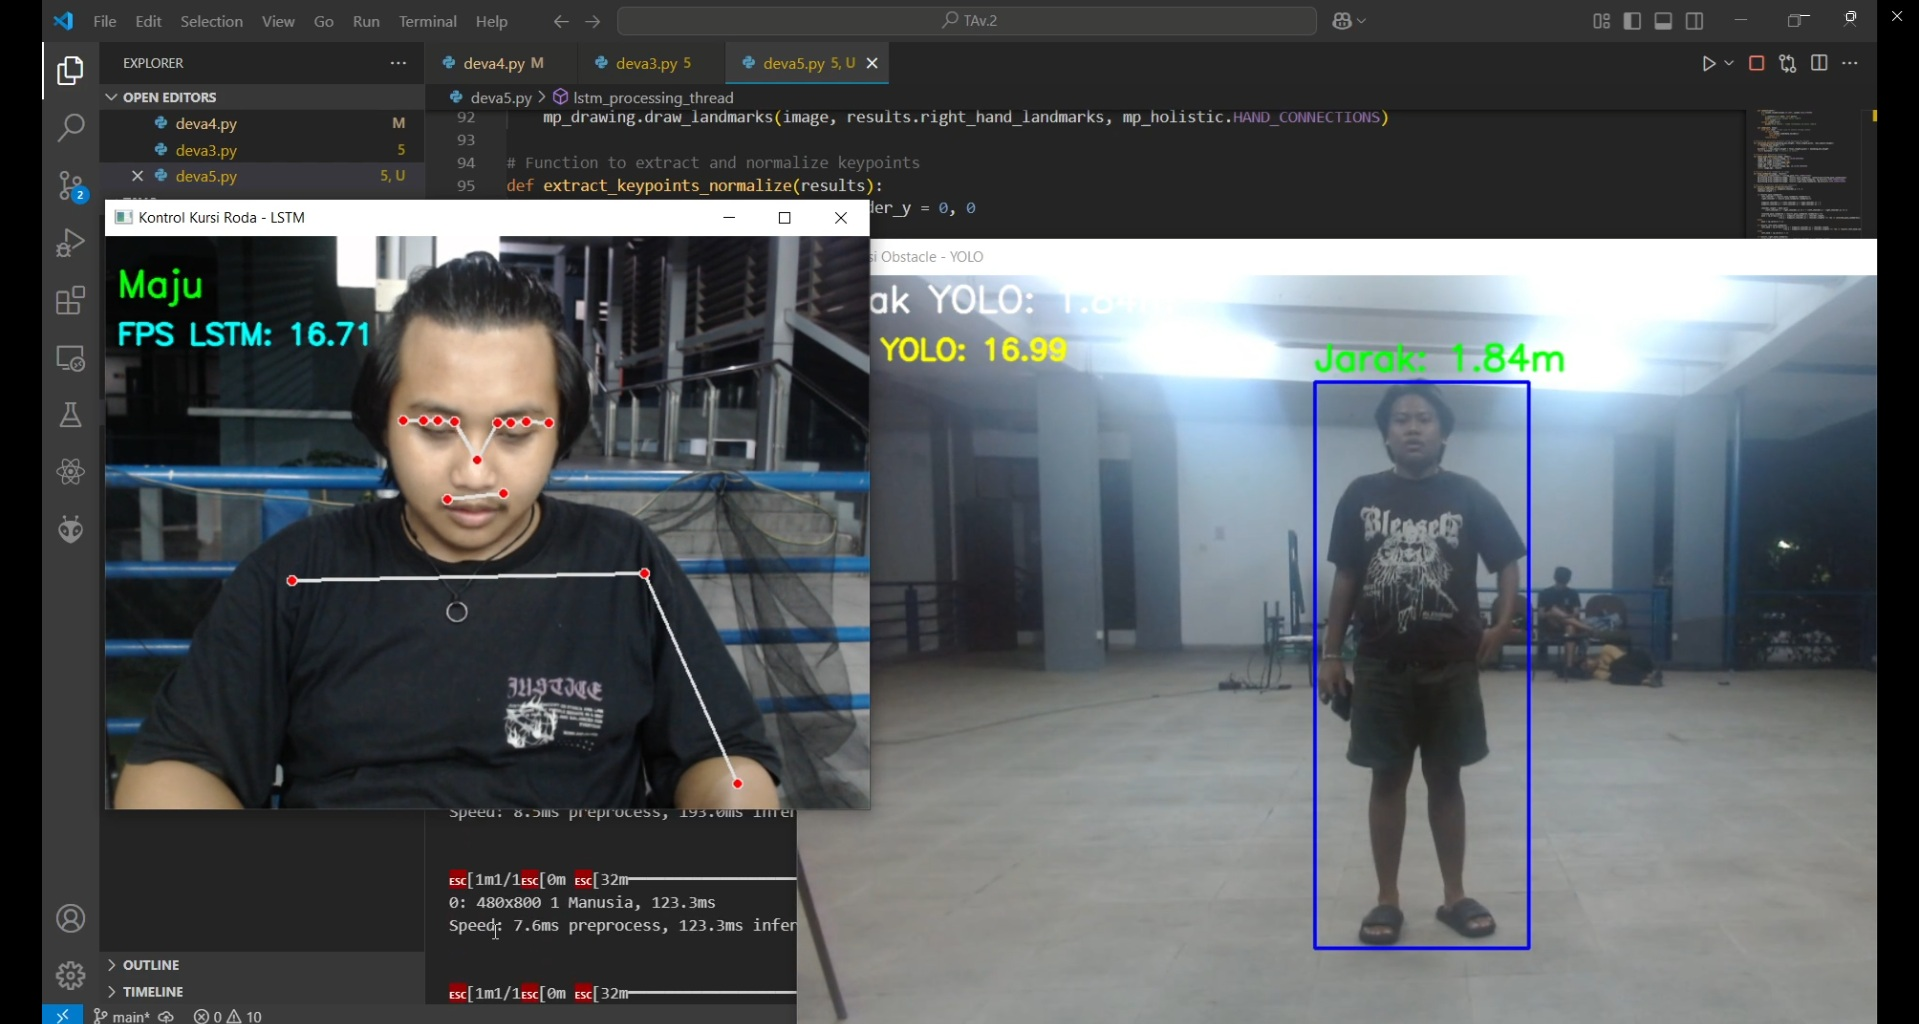
\includegraphics[scale=0.3]{gambar/performakeberhasilan.jpg}
  \caption{Sampel Performa Pengereman Otomatis}
  \label{fig:Fotoperforma}
\end{figure}

Selanjutnya hasil dari performa pengereman otomatis ini dicatat dalam tabel. Agar memudahkan pembaca dalam memahami isi tabel diberikan warna sesuai dengan hasil yang didapatkan. Berikut merupakan hasil pengujian tersebut.

\begin{table}[H]
  \centering
  \caption{Tabel Performa Keberhasilan Pengereman Otomatis menggunakan YOLOv11}
  \label{tb:tabelyolov11performa}
  \begin{tabular}{|c|c|}
  \hline
  Percobaan & Hasil                                                \\ \hline
  1         & \cellcolor[HTML]{34FF34}Kursi Roda Berhasil Berhenti \\ \hline
  2         & \cellcolor[HTML]{34FF34}Kursi Roda Berhasil Berhenti \\ \hline
  3         & \cellcolor[HTML]{34FF34}Kursi Roda Berhasil Berhenti \\ \hline
  4         & \cellcolor[HTML]{34FF34}Kursi Roda Berhasil Berhenti \\ \hline
  5         & \cellcolor[HTML]{34FF34}Kursi Roda Berhasil Berhenti \\ \hline
  6         & \cellcolor[HTML]{34FF34}Kursi Roda Berhasil Berhenti \\ \hline
  7         & \cellcolor[HTML]{34FF34}Kursi Roda Berhasil Berhenti \\ \hline
  8         & \cellcolor[HTML]{34FF34}Kursi Roda Berhasil Berhenti \\ \hline
  9         & \cellcolor[HTML]{34FF34}Kursi Roda Berhasil Berhenti \\ \hline
  10        & \cellcolor[HTML]{34FF34}Kursi Roda Berhasil Berhenti \\ \hline
  \end{tabular}
  \end{table}

Dari hasil yang didapatkan pada tabel \ref{tb:tabelyolov11performa} pada 10 kali sampel percobaan didapatkan rasio keberhasilan sebesar 100\% yang menunjukan bahwa sistem pengereman otomatis menggunakan model YOLOv11 dapat berjalan dengan sempurna.

\begin{table}[H]
  \centering
  \caption{Tabel Performa Keberhasilan Pengereman Otomatis menggunakan YOLOv11}
  \label{tb:tabelyolov8performa}
  \begin{tabular}{|c|c|}
    \hline
    Percobaan & Hasil                                                \\ \hline
    1         & \cellcolor[HTML]{34FF34}Kursi Roda Berhasil Berhenti \\ \hline
    2         & \cellcolor[HTML]{34FF34}Kursi Roda Berhasil Berhenti \\ \hline
    3         & \cellcolor[HTML]{34FF34}Kursi Roda Berhasil Berhenti \\ \hline
    4         & \cellcolor[HTML]{34FF34}Kursi Roda Berhasil Berhenti \\ \hline
    5         & \cellcolor[HTML]{34FF34}Kursi Roda Berhasil Berhenti \\ \hline
    6         & \cellcolor[HTML]{34FF34}Kursi Roda Berhasil Berhenti \\ \hline
    7         & \cellcolor[HTML]{34FF34}Kursi Roda Berhasil Berhenti \\ \hline
    8         & \cellcolor[HTML]{34FF34}Kursi Roda Berhasil Berhenti \\ \hline
    9         & \cellcolor[HTML]{34FF34}Kursi Roda Berhasil Berhenti \\ \hline
    10        & \cellcolor[HTML]{FD6864}Kursi Roda Gagal Berhenti    \\ \hline
    \end{tabular}
  \end{table}

Dari hasil yang didapatkan pada tabel \ref{tb:tabelyolov8performa} pada 10 kali sampel percobaan didapatkan rasio keberhasilan sebesar 90\%. Adapun pada percobaan ke 10 sistem gagal dalam melakukan pengereman otomatis. Hal ini disebabkan oleh 2 faktor yang pertama adalah bounding box yang dihasilkan oleh YOLOv8 tidak sekonsisten YOLOv11, dan yang kedua adalah suhu laptop yang meningkat yang mengurangi performa sistem.

\begin{table}[H]
  \centering
  \caption{Tabel Performa Keberhasilan Pengereman Otomatis menggunakan YOLOv12}
  \label{tb:tabelyolov12performa}
  \begin{tabular}{|c|c|}
  \hline
  Percobaan & Hasil                                                \\ \hline
  1         & \cellcolor[HTML]{34FF34}Kursi Roda Berhasil Berhenti \\ \hline
  2         & \cellcolor[HTML]{34FF34}Kursi Roda Berhasil Berhenti \\ \hline
  3         & \cellcolor[HTML]{34FF34}Kursi Roda Berhasil Berhenti \\ \hline
  4         & \cellcolor[HTML]{34FF34}Kursi Roda Berhasil Berhenti \\ \hline
  5         & \cellcolor[HTML]{34FF34}Kursi Roda Berhasil Berhenti \\ \hline
  6         & \cellcolor[HTML]{34FF34}Kursi Roda Berhasil Berhenti \\ \hline
  7         & \cellcolor[HTML]{34FF34}Kursi Roda Berhasil Berhenti \\ \hline
  8         & \cellcolor[HTML]{34FF34}Kursi Roda Berhasil Berhenti \\ \hline
  9         & \cellcolor[HTML]{34FF34}Kursi Roda Berhasil Berhenti \\ \hline
  10        & \cellcolor[HTML]{34FF34}Kursi Roda Berhasil Berhenti \\ \hline
  \end{tabular}
\end{table}

Dari hasil yang didapatkan pada tabel \ref{tb:tabelyolov12performa} pada 10 kali sampel percobaan didapatkan rasio keberhasilan sebesar 100\% yang menunjukan bahwa sistem pengereman otomatis menggunakan model YOLOv12 dapat berjalan dengan sempurna.

\subsection{Pengujian Akurasi Sistem Pengereman Otomatis}
Untuk mengetahui lebih dalam performa dari model dalam melakukan pengereman maka diperlukannya Uji akurasi dari sistem pengereman otomatis ini. Uji akurasi ini dilakukan dengan cara menghitung jarak yang didapatkan pada sistem dan jarak asli menggunakan meteran. Gambar \ref{fig:FotoPengambilanakurasi} telah dilakukan pengukuran menggunakan meteran untuk mendapatkan jarak saat terjadi pengereman dan juga mengambil jarak pada sistem dengan mendokumentasikan hasil dari sistem dengan menggunakan OBS.

\begin{figure} [H] 
  \centering
  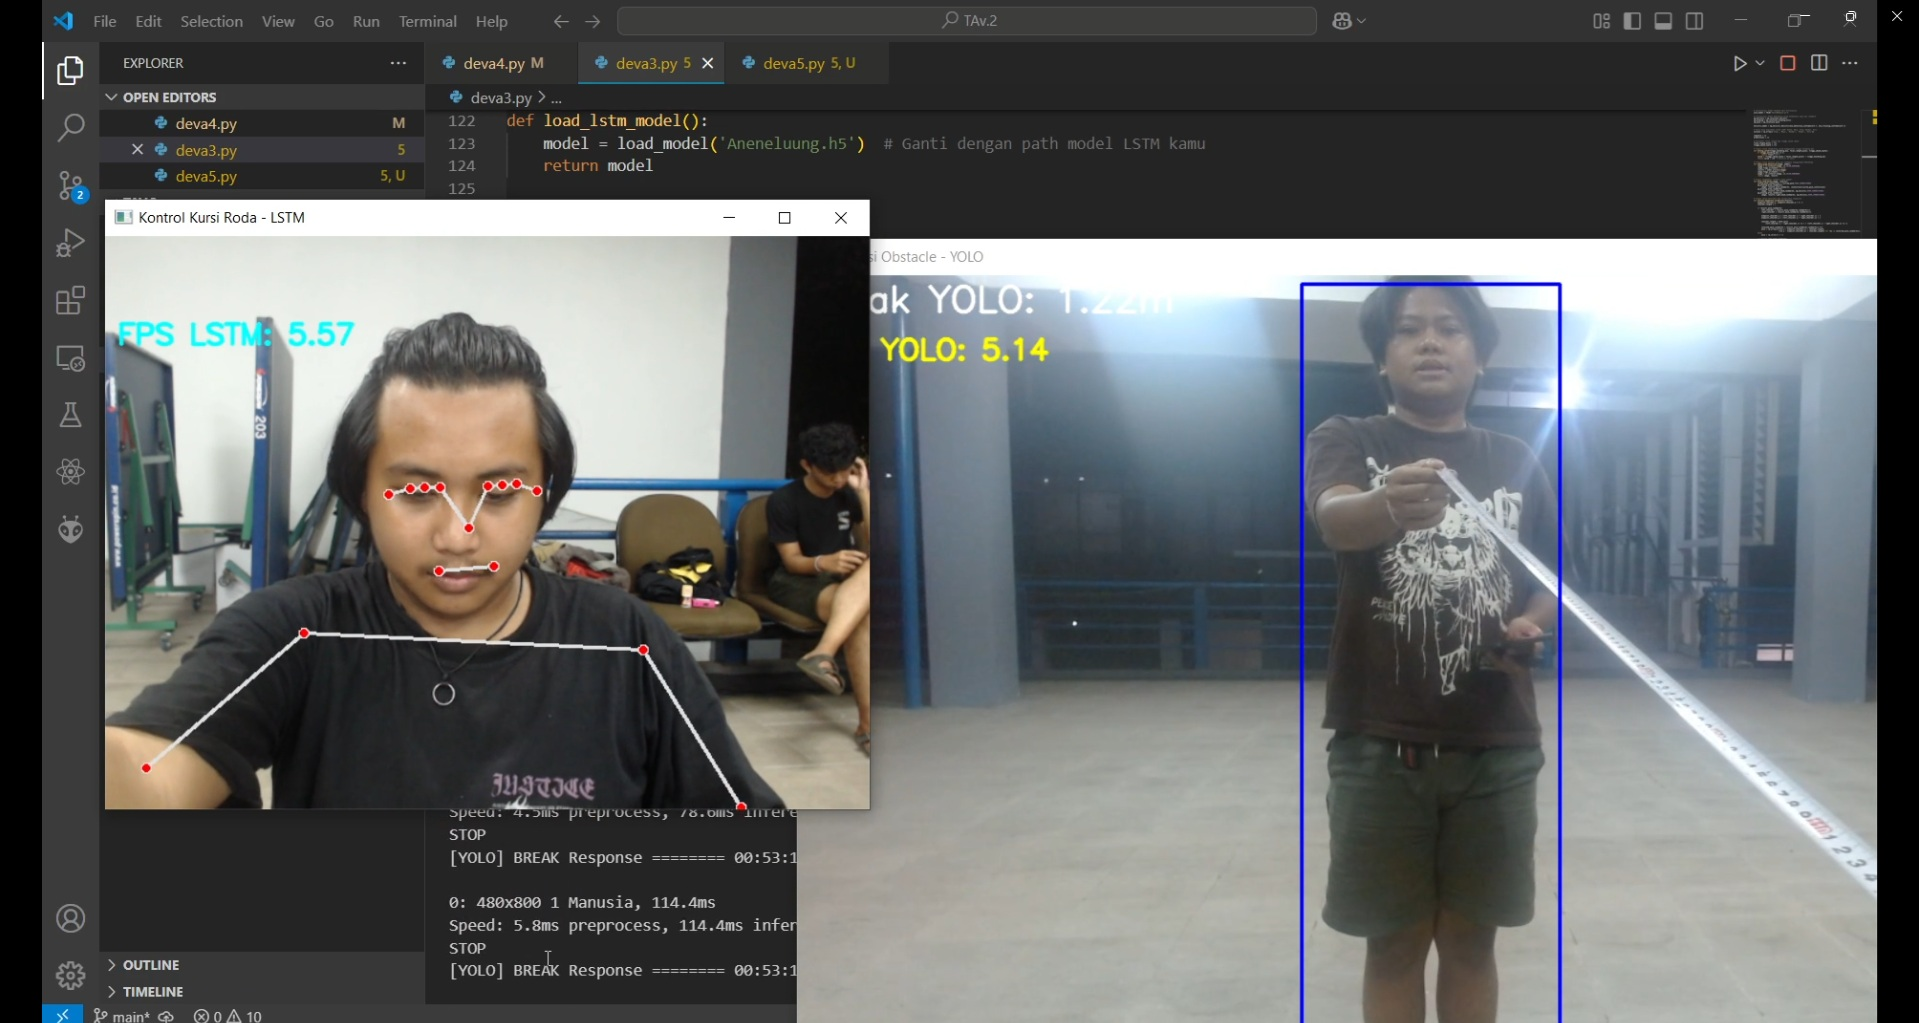
\includegraphics[scale=0.3]{gambar/pengujianjarakdeva.jpg}
  \caption{Hasil Pengukuran Jarak Pengereman Otomatis}
  \label{fig:FotoPengambilanakurasi}
\end{figure}

Jarak yang telah diukur lalu dibandingkan sehingga menghasilkan Tabel \ref{tb:akurasijarak} yang berisi nilai jarak pengukuran nyata saat pengereman (Real Distance), Jarak pada sistem yang telah dicatat (System Distance), Error nyata, dan error sistem. Adapun tujuan dilakukannya pengujian ini yaitu untuk mengetahui kesalahan jarak yang dihasilkan dari sistem dan juga mengetahui penyebab kesalahan pengukuran jarak tersebut.

\begin{table}[H]
  \centering
  \caption{Tabel hasil pengukuran jarak pengereman otomatis}
  \label{tb:akurasijarak}
  \begin{tabular}{|l|l|l|l|l|}
  \hline
  Braking Distance & Real Distance & System Distance & Real Error & System Error \\ \hline
  130\,cm          & 127\,cm        & 125\,cm          & 3\,cm      & 5\,cm        \\ \hline
  130\,cm          & 124\,cm        & 123\,cm          & 6\,cm      & 7\,cm        \\ \hline
  130\,cm          & 115\,cm        & 115\,cm          & 15\,cm     & 15\,cm       \\ \hline
  130\,cm          & 110\,cm        & 110\,cm          & 20\,cm     & 20\,cm       \\ \hline
  130\,cm          & 108\,cm        & 108\,cm          & 22\,cm     & 22\,cm       \\ \hline
  130\,cm          & 112\,cm        & 112\,cm          & 18\,cm     & 18\,cm       \\ \hline
  130\,cm          & 111\,cm        & 111\,cm          & 19\,cm     & 19\,cm       \\ \hline
  130\,cm          & 113\,cm        & 113\,cm          & 17\,cm     & 17\,cm       \\ \hline
  130\,cm          & 104\,cm        & 104\,cm          & 26\,cm     & 26\,cm       \\ \hline
  130\,cm          & 98\,cm         & 99\,cm           & 32\,cm     & 31\,cm       \\ \hline
  \end{tabular}
\end{table}

Dalam uji akurasi pengereman didapatkan hasil yaitu error pengukuran nyata sebesar  17.8 cm dan error sistem sebesar  18.0 cm. Dapat dilihat terdapat peningkatan nilai error yang terjadi pada sistem pengereman otomatis ini, hal tersebut disebabkan oleh beberapa faktor yaitu posisi kamera yang terguncang saat pengujian, delay pada sistem, laptop yang tidak di charge saat pengujian, dan suhu ruangan yang cukup panas menyebabkan laptop menjadi lambat. 